\documentclass[border=10pt]{standalone}
\usepackage[svgnames]{xcolor}
\usepackage{amsmath}
\usepackage{pgfplots}
\pgfplotsset{compat=newest}
\usepackage[sfdefault]{FiraSans}
\usepackage{FiraMono}
\renewcommand*\familydefault{\sfdefault}
\begin{document}
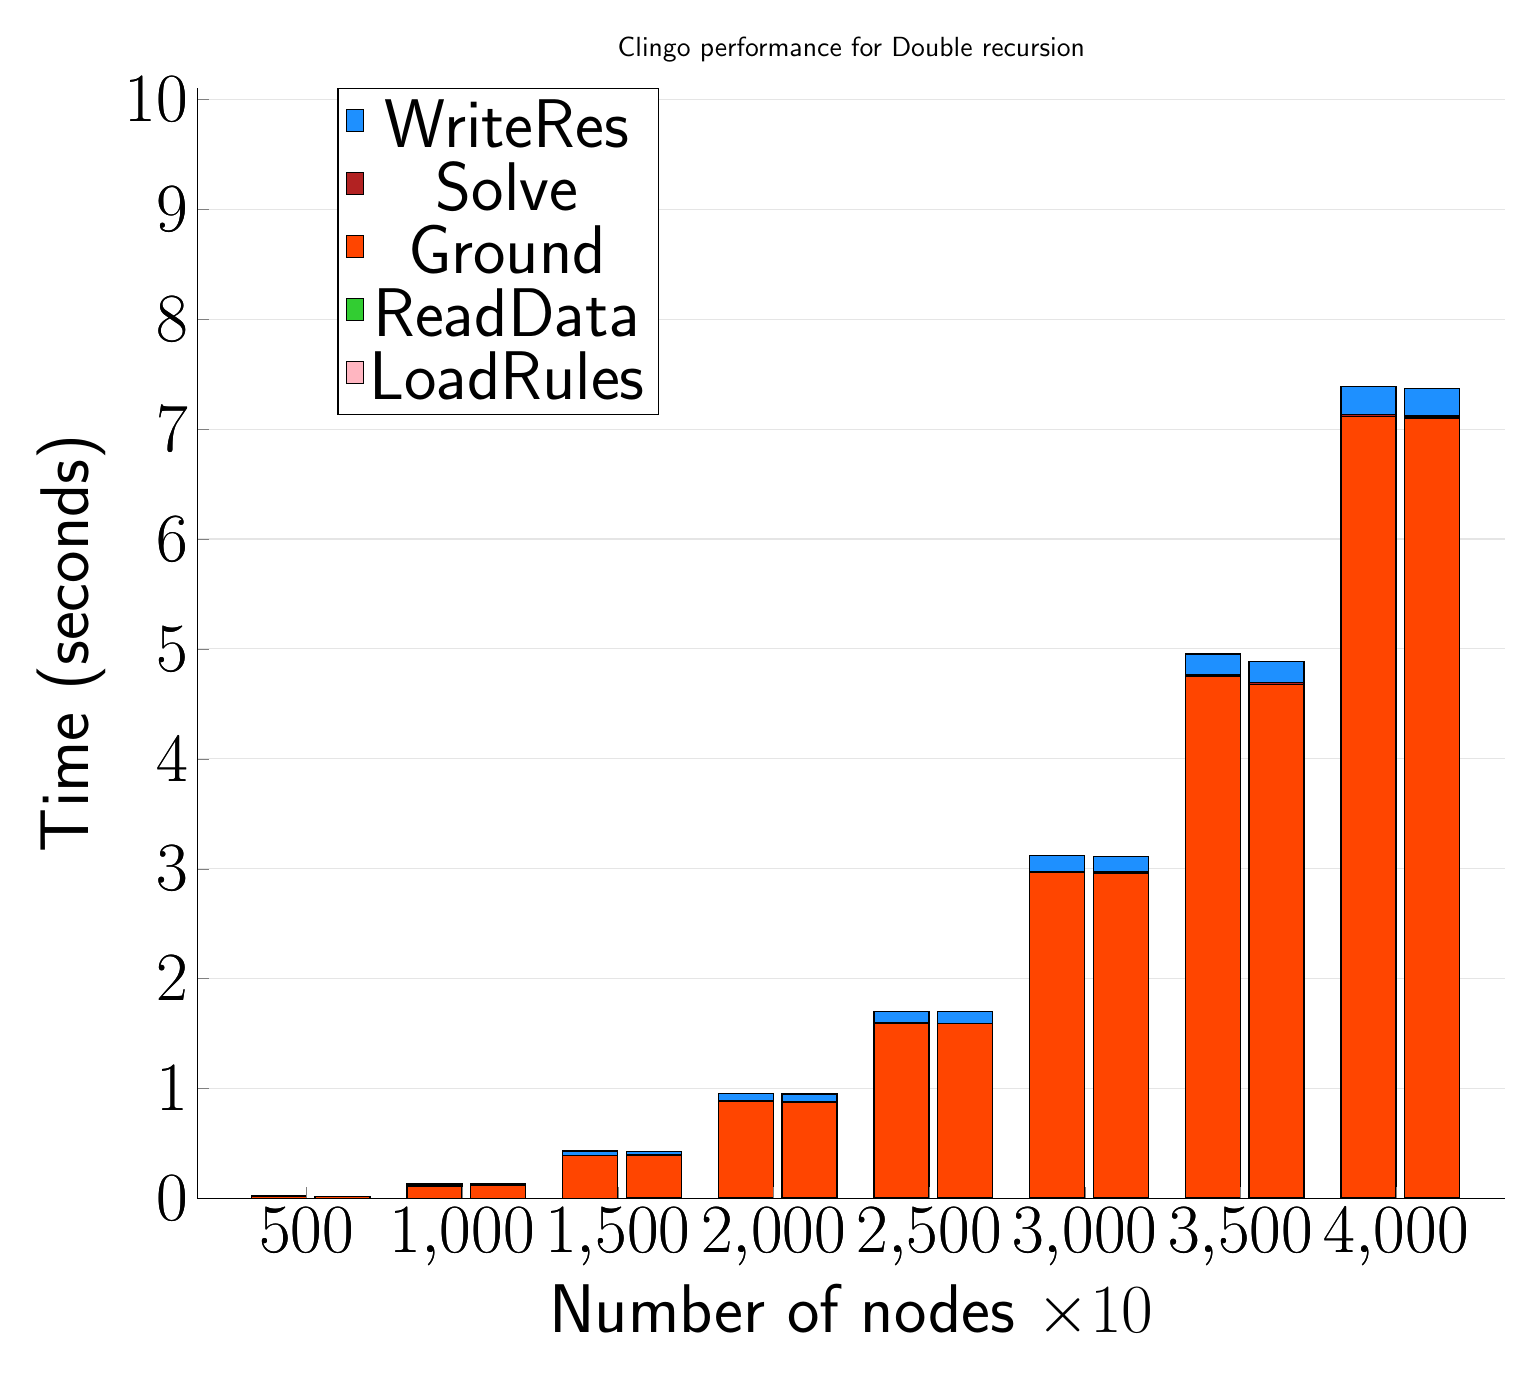
\begin{tikzpicture}
\begin{axis}[
   ybar stacked,
   title={Clingo performance for Double recursion},
   bar shift=-10pt,
   width=1.5\textwidth,
   bar width=0.7cm,
   ymajorgrids, tick align=inside,
   major grid style={draw=gray!20},
   xtick=data,
   ymin=0, ymax=10.104000020027161,
   axis x line*=bottom,
   axis y line*=left,
   enlarge x limits=0.1,
   legend style={
       at={(0.23, 1)},
       anchor=north,
       legend columns=1,
       font=\Huge,
   },
   ylabel={Time (seconds)},
   xlabel={Number of nodes $\times 10$},
   label style={font=\Huge},
   tick label style={font=\Huge},
]
\addlegendimage{fill=DodgerBlue, draw=black, line width=0.2pt}
\addlegendentry{WriteRes}
\addlegendimage{fill=FireBrick, draw=black, line width=0.2pt}
\addlegendentry{Solve}
\addlegendimage{fill=OrangeRed, draw=black, line width=0.2pt}
\addlegendentry{Ground}
\addlegendimage{fill=LimeGreen, draw=black, line width=0.2pt}
\addlegendentry{ReadData}
\addlegendimage{fill=LightPink, draw=black, line width=0.2pt}
\addlegendentry{LoadRules}
\addplot +[fill=LightPink, draw=black, line width=0.5pt] coordinates {
    (500, 0.0)
    (1000, 0.0)
    (1500, 0.0)
    (2000, 0.0)
    (2500, 0.0)
    (3000, 0.0)
    (3500, 0.0)
    (4000, 0.0)
};
\addplot +[fill=LimeGreen, draw=black, line width=0.5pt] coordinates {
    (500, 0.0)
    (1000, 0.0019999980926513673)
    (1500, 0.0020000219345092775)
    (2000, 0.007999992370605469)
    (2500, 0.008999991416931152)
    (3000, 0.007999992370605469)
    (3500, 0.011999988555908203)
    (4000, 0.012000012397766113)
};
\addplot +[fill=OrangeRed, draw=black, line width=0.5pt] coordinates {
    (500, 0.02000002861022949)
    (1000, 0.1119999885559082)
    (1500, 0.3910000085830688)
    (2000, 0.8780000686645508)
    (2500, 1.5860000133514405)
    (3000, 2.9619999647140505)
    (3500, 4.736999988555908)
    (4000, 7.1040000200271605)
};
\addplot +[fill=FireBrick, draw=black, line width=0.5pt] coordinates {
    (500, 0.0)
    (1000, 0.0009999990463256836)
    (1500, 0.0009999990463256836)
    (2000, 0.0029999971389770507)
    (2500, 0.0029999971389770507)
    (3000, 0.007000041007995605)
    (3500, 0.015000033378601074)
    (4000, 0.01399998664855957)
};
\addplot +[fill=DodgerBlue, draw=black, line width=0.5pt] coordinates {
    (500, 0.0019999980926513673)
    (1000, 0.01700000762939453)
    (1500, 0.03899998664855957)
    (2000, 0.06599993705749511)
    (2500, 0.10500004291534423)
    (3000, 0.14599995613098143)
    (3500, 0.18999993801116943)
    (4000, 0.2580000162124634)
};
\end{axis}
\begin{axis}[
   ybar stacked,
   bar shift=13pt,
   width=1.5\textwidth,
   bar width=0.7cm,
   ymajorgrids, tick align=inside,
   major grid style={draw=none},
   xtick=data,
   ymin=0, ymax=10.104000020027161,
   axis x line*=none,
   axis y line*=none,
   enlarge x limits=0.1,
   label style={font=\Huge},
   tick label style={font=\Huge},
]
\addplot +[fill=LightPink, draw=black, line width=0.5pt] coordinates {
    (500, 0.0)
    (1000, 0.0)
    (1500, 0.0)
    (2000, 0.0)
    (2500, 0.0)
    (3000, 0.0)
    (3500, 0.0)
    (4000, 0.0)
};
\addplot +[fill=LimeGreen, draw=black, line width=0.5pt] coordinates {
    (500, 0.0)
    (1000, 0.0)
    (1500, 0.009999999999999997)
    (2000, 0.008999999999999998)
    (2500, 0.009999999999999997)
    (3000, 0.009999999999999997)
    (3500, 0.010999999999999998)
    (4000, 0.009999999999999997)
};
\addplot +[fill=OrangeRed, draw=black, line width=0.5pt] coordinates {
    (500, 0.019999999999999997)
    (1000, 0.11800000000000002)
    (1500, 0.383)
    (2000, 0.8709999999999999)
    (2500, 1.5800000000000003)
    (3000, 2.9519999999999995)
    (3500, 4.667999999999999)
    (4000, 7.0920000000000005)
};
\addplot +[fill=FireBrick, draw=black, line width=0.5pt] coordinates {
    (500, 0.0)
    (1000, 0.0020000000000000018)
    (1500, 0.002999999999999997)
    (2000, 0.0)
    (2500, 0.0020000000000000018)
    (3000, 0.009999999999999943)
    (3500, 0.013000000000000123)
    (4000, 0.016000000000000014)
};
\addplot +[fill=DodgerBlue, draw=black, line width=0.5pt] coordinates {
    (500, 0.0)
    (1000, 0.010999999999999992)
    (1500, 0.032000000000000015)
    (2000, 0.07199999999999998)
    (2500, 0.10799999999999992)
    (3000, 0.14200000000000007)
    (3500, 0.19499999999999976)
    (4000, 0.24900000000000003)
};
\end{axis}
\end{tikzpicture}

\end{document}
